% This must be in the first 5 lines to tell arXiv to use pdfLaTeX, which is strongly recommended.

% In particular, the hyperref package requires pdfLaTeX in order to break URLs across lines.

\documentclass[11pt]{article}
\pdfoutput=1
% Remove the "review" option to generate the final version.
\usepackage{ACL2023}
\usepackage{caption}
% Standard package includes
\usepackage{times}
\usepackage{latexsym}
\usepackage{graphicx}
\usepackage{amsmath}
% For proper rendering and hyphenation of words containing Latin characters (including in bib files)
\usepackage[T1]{fontenc}
% For Vietnamese characters
% \usepackage[T5]{fontenc}
% See https://www.latex-project.org/help/documentation/encguide.pdf for other character sets

% This assumes your files are encoded as UTF8
\usepackage[utf8]{inputenc}

% This is not strictly necessary, and may be commented out.
% However, it will improve the layout of the manuscript,
% and will typically save some space.
\usepackage{microtype}

% This is also not strictly necessary, and may be commented out.
% However, it will improve the aesthetics of text in
% the typewriter font.
\usepackage{inconsolata}


% If the title and author information does not fit in the area allocated, uncomment the following
%
%\setlength\titlebox{<dim>}
%
% and set <dim> to something 5cm or larger.

\title{Comparative Study of Binary Sentiment Analysis for the Product Review dataset with the Explainable AI framework} 

\author{Dimitra Muni\\
  732A92 - Text Mining \\
  Linköping University \\
  \texttt{dimmu472@student.liu.se}
  }
\begin{document}

\maketitle
\begin{abstract}
This project aimed to analyze binary sentiment for the Amazon Fine Food Reviews dataset\footnote{\url{https://snap.stanford.edu/data/web-FineFoods.html}} using different vectorization and word embedding techniques and evaluated the performance on the gold standard dataset. In the first part of the project, we utilized two different word vectorization (i.e. count  and TF-IDF vectorizers) techniques in conjunction with three linear classifiers (i.e. Multinomial Naive Bayes, Logistic Regression, and Support Vector Machine (SVM) ) to create six experimental pipelines. Furthermore, we used the \textit{Halving Grid Search} technique to find the best-performing model with five-fold cross-validation. Here SVM slightly outperformed the other two models with an accuracy of 93\%. In the second part of the project, we utilized pre-trained DistilBERT to perform sentiment classification on a smaller subset of original data; without fine-tuning, it achieved 85\% accuracy, but the performance was not as high as the SVM model. In the third part of the project, we performed LIME \cite{LIME} analysis for a subset of misclassified samples identified from the final SVM model and documented actionable insights.
\end{abstract}

\section{Introduction}
In the last decade, massive development in Masked Language Models has opened the floodgates of possibility in Natural Language Processing (NLP) domain. 
\textbf{B}idirectional \textbf{E}ncoder \textbf{R}epresentations from \textbf{T}ransformers (BERT), developed by \cite{BERT} at Google, is one such model. The base version of BERT has 110 million parameters and is computationally expensive to train. Several variants of this model, such as DistilBERT \cite{distilbert} with 66 million parameters, is significantly faster than the base version of BERT; however, with a decline in performance.

In this project, we focus on the problem of binary sentiment analysis for the Amazon Fine Foods dataset, which contains product reviews collected over a decade. We intend to address the following research objectives,
\begin{enumerate}
    \item Experiment with word vectorizer-based technique with machine learning classifiers to perform sentiment classification.
    
    \item Investigate the applicability of the compact Masked Language Model (MLM) for sentiment classification.
    
    \item Inference about misclassified samples obtained from the best-performing model, generating actionable insight using an explainable AI technique.
\end{enumerate}
In the initial part of this project, we created six different vectorizer-classifier pipelines, using two vectorizers and three classifiers; we utilized a halving grid search technique with five-fold cross-validation to tune these pipelines and evaluated the performance on the test set. In the second part of the project, we trained the DistilBERT model for ten epochs and evaluated the performance on the test set. 
In the last part of the project, we focus on the misclassified samples (from the test set) identified using the Linear SVM model. We used a popular explainable AI technique called LIME analysis \cite{LIME} to perform this study.

 \section{Theory}
\subsection{Vectorization}
The vectorization technique converts the corpus of text data into a matrix representation; one such technique is Count Vectorizer, which uses a \textit{bag-of-word} representation \cite{jurafsky}. Here the corpus is assumed to be a collection of words, where a matrix represents the frequency of the word \textit{w} in document \textit{d}. A major  constraint of this representation is that the word's position in a sentence is not inconsequential; rather, the frequency of the word is important \cite{jurafsky}. 
Another more advanced method of vectorization is \textit{TF-IDF}; here, \textit{TF} refers to the \textbf{term frequency}, which accounts for the occurrence of the term \textit{t} in document \textit{d}, while \textit{IDF} is \textbf{inverse document frequency}, a measure of the number of documents a term \textit{t} appears. One noteworthy advantage of TF-IDF representation is that it assigns relevance to rare occurring words by higher IDF value \cite{info-ret}.

\subsection{Classifiers}
\subsubsection{Multinomial Naive Bayes}
Multinomial Naive Bayes classifier is based on Bayes' rule \cite{bayes}\footnote{Bayes' rule for two events x and y is presented as in term of conditional probability, $p(x|y)p(y)=p(y|x)p(x)$.} about the conditional probability of two events. This classifier is often a preferred  baseline evaluation method due to its simplicity. According to Jurafsky and Martin (p.61, 2023), there is a \textbf{naive} assumption about conditional independence of the feature probability given the class.

\subsubsection{Logistic Regression}
According to Bishop and Nasrabadi (p.205, 2006), the logistic regression classifier is one of the linear classifier models that uses \textit{logistic sigmoid} function\footnote{logistic sigmoid: $\sigma(a)=\frac{1}{1+\exp{(-a)}}$} for binary classification, minimizing cross-entropy loss. One advantage of this method is that for the correlated features in the dataset, the logistic regression classifier is preferred over naive Bayes because the logistic regression can assign the weights more efficiently amongst the correlated features; while this mechanism is not present in the naive Bayes model (Jurafsky and Martin (p.86, 2023)); due to this reason, we intend to use this model in our experiments.

\subsubsection{Support Vector Machines}
Support Vector Machine (SVM) classifier originally presented by \cite{vapnik} belongs to the class of \textit{maximum margin classifiers} \cite{bishop}, where the objective is to find a hyperplane that separates two classes with the highest margin. There are several variations of SVM classifiers based on the kernel function. However, we only consider the Linear SVM classifier; this method is appropriate for datasets with high dimensions if the dataset has considerably more samples than the number of features; for this reason, we include this method in our analysis.

\subsection{Masked Language Model}
According to \cite{BERT}, the BERT model is trained using a \textit{masked language modeling} technique, where a model is trained by hiding randomly chosen tokens and is asked to predict that token. This model introduces bidirectional context to the training of transformer-based architecture using the attention mechanism \cite{attention}. The BERT model is trained in two iterations; the first iteration is called \textbf{pre-training}, where the model is trained on unlabeled data, and the second is \textbf{fine-tuning}, where the model is tuned on labeled data. This model uses WordPiece embedding \cite{wordpiece}, which converts a word into sub-word units.

In figure [\ref{fig:BERT_archi}], the pre-training and fine-tuning procedure is represented, where a sentence pair is separated by \texttt{[SEP]} token, and before each sentence, there is a classification token \texttt{[CLS]}. Input embedding is denoted by \textbf{\textit{E}}, and \textbf{\textit{C}} represents the final vector corresponding to \texttt{[CLS]} token, and $T_1, T_2, ..., T_N$ represents tokens' final vector representation, where \textit{N = 768} for the BERT-base model.  

\begin{figure*}
\label{fig:BERT_embedding}
    \centering
    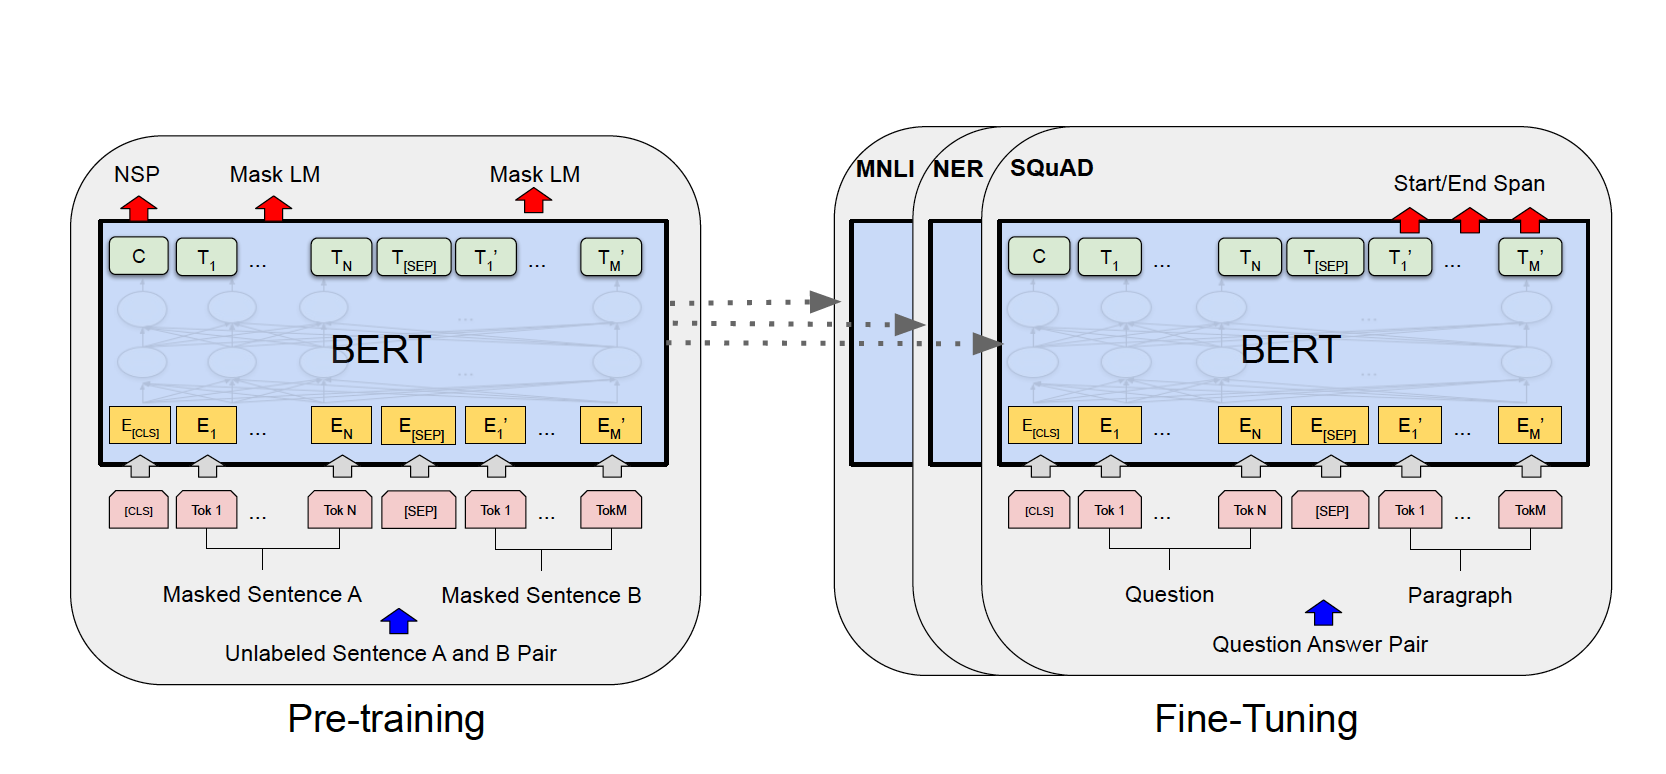
\includegraphics[scale=0.6]{figures/BERT-embedding.png}
    \caption{Pre-training and Fine tuning procedure in BERT, the figure taken from Devlin et al. (p.3, 2019)}
    \label{fig:BERT_archi}
\end{figure*}


\subsubsection{DistilBERT}
DistilBERT, introduced by \cite{distilbert}, is another example of a compact model, with the number of layers reduced by half\footnote{Additionally token-type embedding and pooler are removed as well.}, and has a similar architecture to that of a BERT-base model, as indicated in the table [\ref{tab:bert_distil}].
 \begin{table}[h!]
 \scriptsize
     \centering
     \begin{tabular}{c c c c c}
     \hline 
        \textbf{Model} & \textbf{No. of}  & \textbf{Hidden} & \textbf{Attention} & \textbf{Parameters} \\
        &\textbf{Layers}& \textbf{Size} & \textbf{Heads} & \textbf{(millions)} \\
        \hline 
         {BERT-base} &12 &768 &12&110 \\
         {DistilBERT} & 6& 768& 12&66\\    
         \hline   
     \end{tabular}
     \caption{BERT and DistilBERT model Architecture Comparision}
     \label{tab:bert_distil}
 \end{table}
According to \cite{smallBERT}, knowledge distillation is the technique \cite{kdistillation},  where a bigger teacher model transfers the knowledge to a more compact model.


\textbf{Triple Loss:}
Authors trained DistilBERT using a linear combination of three loss functions, cross-entropy distillation loss ($L_{ce}$), masked language modeling loss ($L_{mlm}$), and cosine embedding loss ($L_{cos}$) calculated by performing cosine operation on a hidden vector of student and teacher.

According to \cite{distilbert} \textbf{DistilBERT} is significantly faster (60\%) and smaller (40\%) than BERT-base. The authors evaluated DistilBERT for the sentiment classification task on the IMDb dataset, and it performed almost at par (accuracy of 92.82) with BERT-base (accuracy of 93.46). We intend to investigate the usage of DistilBERT for a similar task but with the Amazon Fine Foods dataset.
\subsection{LIME}
\textbf{L}ocal \textbf{I}nterpretable \textbf{M}odel agnostic \textbf{E}xplanation (LIME) \cite{LIME} is a popular explainable AI framework to understand the underlying pattern that black box models are trained with and for the inference about the predictions. LIME perturbs the black-box model, observes local changes, and provides a visual explanation for greater understanding. LIME is model agnostic, i.e. it can be used for any model and provide explanations.


 \section{Data}
 \label{sec:data}
 We have chosen the Amazon Fine Foods dataset hosted on the \href{https://snap.stanford.edu/about.html}{SNAP library} affiliated with Stanford University. This dataset contains reviews of 74,258 unique products and 568,454 product reviews by 256,059 users, collected between October 1999 and October 2012.
 
 The features of this dataset are described in the table [\ref{feat-description}].
 \begin{table}[h!]
 \scriptsize
    \centering
     \begin{tabular}{c c}
     \hline
          \textbf{Feature} & \textbf{Description}\\ \hline 
     productId &\href{https://en.wikipedia.org/wiki/Amazon_Standard_Identification_Number}{ASIN} - Amazon Standard \\
     & Identification Number\\ 
          userId & reviewer identification \\
          profileName & reviewer profile name\\
          helpfullness & fraction of users\\
          & who found the review helpful\\
          score & score from 1 to 5\\
          time &time of review post\\
          summary&review summary \\ 
          text & review text\\   \hline
     \end{tabular}
     \caption{Feature Description for Amazon Fine Food dataset}
     \label{feat-description}
 \end{table}
 Our analysis focused on the \textit{text} and \textit{score} variables. Firstly, in figure [\ref{fig:review_score_distri}], the distribution of review score is presented, where the dataset had a class imbalance, with a higher number of reviews with a score of 5. 
\begin{figure}[h!]
     \centering
     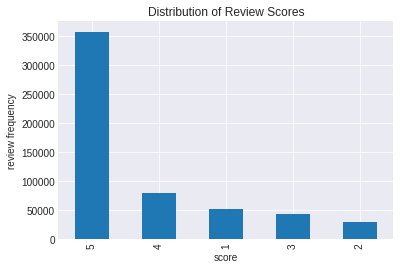
\includegraphics[scale=0.5]{figures/distribution_review_score.png}
     \caption{Distribution of Review Scores}
     \label{fig:review_score_distri}
 \end{figure}
  
  \begin{table}[h!]
 \scriptsize
     \centering
     \begin{tabular}{c| c c | c c}
     & Before &Undersampling& After& Undersampling \\
     \hline 
        \textbf{Type} & \textbf{Positive} & \textbf{Negative} &\textbf{Positive} &\textbf{Negative}\\ \hline 
         Train &  371989 &68965 &68965 & 68965\\
          Test & 65646 &12170 & 65646 &12170\\ \hline 
     \end{tabular}
     \caption{Distribution of Positive and Negative Class before and after Undersampling}
     \label{tab:class_distri}
 \end{table}
 As we intend to perform a binary classification of the review dataset, the newly engineered dataset disregards the reviews with a score of 3, and the reviews with scores 1 and 2 are encoded with binary value '1' and reviews with scores 4 and 5 are encoded with '0'. After performing the aforementioned encoding, the dataset has 371,989 reviews with values '1' (positive reviews) and 68,965 reviews with values '0' (negative reviews); if we train our model with the imbalanced dataset, the results would be incorrect and untrustworthy. To mitigate this problem, we perform random undersampling using the \texttt{imblearn} python package, so the final dataset would have 68,965 reviews with positive and negative reviews classes each, as described in the table [\ref{tab:class_distri}].

 
 \section{Method} 
 The workflow of this project is visualized in figure \ref{fig:workflow}. We have utilized python packages such as \textbf{scikit-learn} \cite{scikit-learn}, \textbf{imbalanced-learn} \cite{imblearn}, \textbf{NumPy} \cite{numpy}, \textbf{Pandas} \cite{pandas} \cite{pandassoft} and \textbf{Matlplotlib} \cite{matplotlib}.
 \begin{figure}
     \centering
     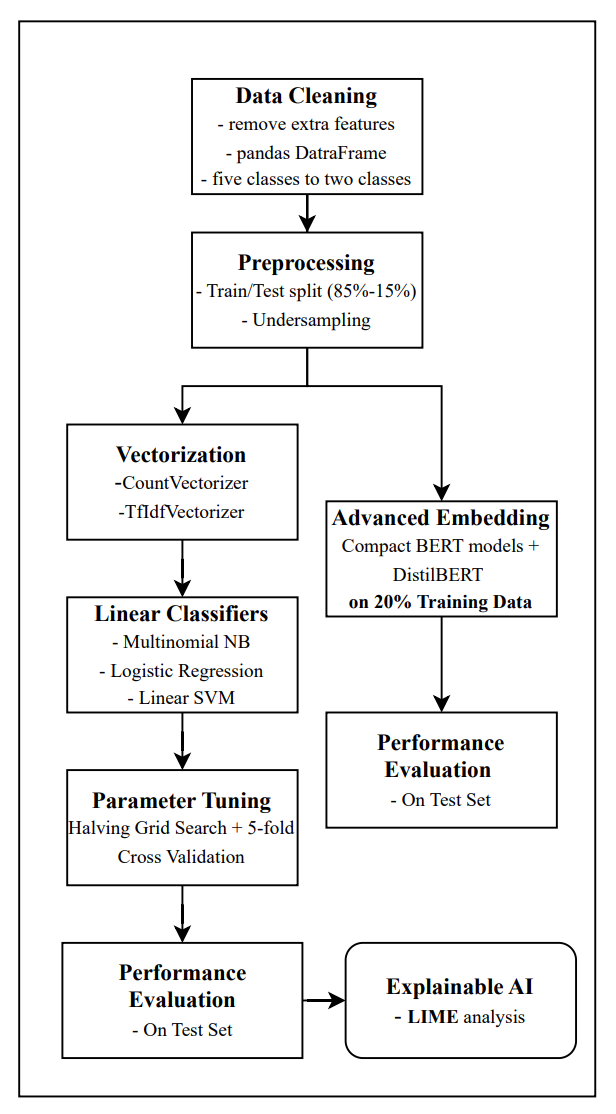
\includegraphics[scale=0.5]{figures/TM-workflow.png}
     \caption{Workflow of the Project}
     \label{fig:workflow}
 \end{figure}

 \subsection{Data Cleaning}
The FineFoods dataset was scraped by \cite{finefoods}. The dataset is available in \texttt{txt.gz} format. The data-cleaning procedure is described as follows,
\begin{enumerate}
    \item Created a raw list\footnote{Using Google Colab with python3 distribution.} from the textual data. Converted this list of rows into a dictionary, disregarded extra features if the raw has more than eight features. The dictionary was converted to a \texttt{pandas} data frame.
    \item Finally, we converted the five-class classification problem into a binary classification problem, as documented in section [\ref{sec:data}].
\end{enumerate}
 \subsection{Preprocessing}
In the preprocessing part, first, we converted the dataset from the previous step into training and test sets using \texttt{train\_test\_split} \footnote{Available from \texttt{sklearn.model\_selection}} function from \texttt{sklearn} library, here the train-test split was selected to be 85\%-15\%. We used \textit{stratify} option to maintain the same proportion of class division in training and test sets.

Furthermore, the class imbalance problem in the training dataset was addressed using \texttt{RandomUnderSampler}\footnote{Available from the \texttt{imblearn.under\_sampling} module} from the \texttt{imblearn} library. The final training dataset has a 50\%-50\% division between positive and negative classes.

\subsection{Vectorizer-Classifier Pipeline}
We have used two vectorizers and three classifiers, as shown in the table [\ref{tab:vectorizer_paras}] and [\ref{tab:classfiers_para}], and set up six ($2 * 3$) pipelines using \texttt{Pipeline} function from the \texttt{sklearn.pipeline} module. 

 \begin{table}[h!]
\scriptsize
     \centering
     \begin{tabular}{c|c}
     \hline 
         \textbf{Vectorizer} & \textbf{Parameters}  \\ \hline 
          Count Vectorizer & ngram\_range: [(1,1),(1,2),(1,3)]\\
          and & encoding:'latin-1'\\
          TF-IDF Vectorizer & stop\_words: 'english' \\
          \hline 
     \end{tabular}
     \caption{Vectorizer with the parameters}
     \label{tab:vectorizer_paras}
 \end{table}
We utilized the functions \texttt{CountVectorizer} and \texttt{TfidfVectorizer} from \texttt{sklearn.feature\_extraction} module. We chose three different \textbf{n-gram} variations as indicated in table [\ref{tab:vectorizer_paras}], these are the \textit{unigram}, \textit{unigram + bigram} and \textit{unigram + bigram + trigram}.
Additionally, we choose \texttt{'latin-1'} encoding and remove the stop words using \texttt{stop\_words} command.
\begin{table}[h!]
\scriptsize
    \centering
    \begin{tabular}{c|c}
    \hline
   \textbf{Classifier} & \textbf{Parameter} \\ \hline 
     Multinomial NB & alpha: [1e-3,0.4, 0.8, 1,10] \\ 
      Logistic Regression &  C: [1e-3, 1e-2, 1e-1, 1, 10] \\
      Linear SVM & C: [1e-3, 1e-2, 1e-1, 1, 10] \\\hline 
    \end{tabular}
    \caption{Classifier with the grid of parameters}
    \label{tab:classfiers_para}
\end{table}
We have utilized three classifiers functions from \texttt{sklearn} library using \texttt{MultinomialNB}, \texttt{LogisticRegression} and \texttt{LinearSVC} functions\footnote{These functions are available from \texttt{naive\_bayes}, \texttt{linear\_model} and \texttt{svm} modules accordingly.}.

Here \texttt{MultinomialNB} function is optimized for the smoothing parameter \texttt{alpha}. While \texttt{LogisticRegression} (LR) is optimized on the regularization parameter \texttt{C}, furthermore, as this model utilizes the gradient descent method to update the weight vectors, we set the maximum number of iterations (\texttt{max\_iter=100,000}) \footnote{Based on our primary experiments we realized that this model takes the considerably higher number of iterations before it converges.}. We utilize \texttt{lbfgs} solver \cite{lbfgs} for its robustness\footnote{\url{http://users.iems.northwestern.edu/~nocedal/lbfgsb.html}}. Thirdly we employ the \texttt{LinearSVC} function with the maximum number of iterations as \texttt{max\_iter=100,000} with setting the seed\footnote{In order to reproduce the same results, we set the seed variable as \texttt{random\_state=1729} for \texttt{LogisticRegression} and \texttt{LinearSVC} functions.}.

\subsection{Halving Grid Search with Cross Validation}
\label{met:halving_grid}
Tuning the parameters for six vectorizer-classifier pipelines is an expensive task, considering the fact that the training dataset is relatively large, with 137,930 training samples; furthermore, we intend to perform a grid search on several combinations. To give a perspective, these six pipelines perform a grid search on 15 combinations of parameters.

Here, a conventional grid search technique might not be a time-optimal solution. Therefore, we approach this problem by utilizing the Halving Grid Search method, based on the Successive Halving (SH) technique  (\cite{halving_gs1} and \cite{halving_gs2}. This method is based on the tournament of candidates. Initially, all the candidate models are trained on a smaller dataset; out of these, the best-performing candidates survive and are further trained on a larger dataset  iteratively, and the parameter space of the candidates keeps shrinking. Finally, the best-performing model is found.

We have used the \texttt{HalvingGridSearchCV} function available from \texttt{sklearn.model\_selection} module; this function has parameters such as \texttt{factor} and \texttt{min\_resource}. According to the \href{https://scikit-learn.org/stable/modules/grid_search.html#id4}{documentation}, the parameter \texttt{factor} is the rate at which the number of training samples grows or the rate of reduction for the candidates. Here \texttt{min\_resource} refers to the number of available samples in the first iteration.

In our experiments, we have chosen the value for \texttt{min\_resource = 34,480} and \texttt{factor = 2} because in $3^{rd}$ iteration value of \textbf{n\_resource} will grow to be \textbf{137,920} training samples, while the total training samples is \textbf{137,930}, so in the last iteration, the model will be able to perform the evaluation on almost entire training dataset to find the best-performing candidate out of the four models. 
\begin{table}
    \centering
    \scriptsize
    \begin{tabular}{c c c}
    \hline 
      \textbf{iteration}   & \textbf{n\_resource}  & \textbf{no. of candidates} \\ \hline 
        1 & 34,480 & 15\\
        2 & 68,960 & 8\\
        3 & 137,920 & 4\\\hline     
    \end{tabular}
    \caption{Halving Grid Search Parameters}
    \label{tab:my_label}
\end{table}

We have chosen to five-fold cross-validation for better regularization. Finally, we re-train the best-performing model obtained on the entire data set with the corresponding parameters for further inference in the next stage; here, we use the \texttt{CalibratedClassifierCV} function, as the \texttt{LinearSVC} does not provide probabilities associated with each class in the prediction, we utilized the \href{https://scikit-learn.org/stable/modules/generated/sklearn.calibration.CalibratedClassifierCV.html#sklearn.calibration.CalibratedClassifierCV}{\texttt{CalibratedClassifierCV}} function to obtain the probability associated with each class for the LIME analysis.


\subsection{DistilBERT Training} 
DistilBERT model is faster to train than base-BERT, but still, it is time expensive computation even on TPU v2, so we first train these models on the 20\% subset of training data. This 20\% subset is further divided into train-validation sets with a split of 75\%-25\% to compute the epoch-wise loss and accuracy. Pre-trained DistilBERT is used to build a classifier, using TensorFlow interface \cite{tensorflow}and Keras \cite{keras} package on the Google Colab environment with python3 distribution. We list the steps involved in this process here,
\begin{enumerate}
    \item We installed the \texttt{tensorflow}, and \texttt{tensorflow-text} version \texttt{2.9.0} in the python3 environment\footnote{Ancilliary packages such as \texttt{tensorflow\_text} and \texttt{tensorflow\_hub} are installed.}. The pre-trained DistilBERT model is used to build the classifier using the corresponding \texttt{preprocesser} and the \texttt{encoder} on TensorFlow Hub. 
    \item Next, the \texttt{pooled\_output} from encoded text is passed through a \texttt{Dropout} layer with a rate of 0.1 to control overfitting. The last layer is a \texttt{Dense} layer with a neuron that uses a \texttt{sigmoid} activation function, which has output 0 or 1.

 \item We trained the models for \texttt{epochs=10} with \texttt{batch\_size=256}. We trained the models by using adam optimizer \cite{adam} with 0.001 learning rate and \texttt{binary\_crossentropy }loss. To minimize the training time, the training was performed on a subset (20\%) of the original training data, which was further split into training and validation sets with a split of (75\%-25\%). Finally, we evaluated the performance of this model on the test set.

\end{enumerate}

\subsection{LIME Inference}
The misclassified samples identified by the tuned Linear SVM model using are utilized for the LIME inference. We utilized \texttt{LimeTextExplainer} module from the \texttt{lime\_text} and \texttt{lime} modules.
 
 \section{Results}

\subsection{Vectorizer-Classifier Pipeline}

The classification report for the  pipelines created using Count Vectorizer is represented in table [\ref{tab:cvec_class_report}]; here, all three classifiers seem to perform equally well. However, Linear SVM has slightly higher precision for the negative class.
\begin{table*}
\scriptsize
\centering
    \begin{tabular}{c c c c c c c}
    \hline
       \textbf{Classifier}& \textbf{Class} & \textbf{Precision} &  \textbf{Recall} & \textbf{F1-score}  & \textbf{Accuracy} & \textbf{Tuned Parameters} \\ \hline 
       Multinomial NB & negative &0.67 &0.91 &0.78& &n\_gram: (1,3)  \\
       & positive &0.98&0.92& 0.95 & 0.92 & alpha: 0.8\\ \hline 
       Logistic Regression & negative &0.69& 0.93& 0.79 & & n\_gram: (1,3)\\
       & positive&0.99 &0.92 &0.95&0.92 & C:1\\ \hline 
       Linear SVM & negative& 0.70& 0.92& 0.79 & &  n\_gram: (1,3)\\ 
       & positive & 0.99&0.93 &0.95&0.93 & C: 0.1\\ \hline 
    \end{tabular}
    \caption{Classification Report for the experiment with Count Vectorizer Pipeline + Classifier Pipelines, with Halving Grid Search CV}
    \label{tab:cvec_class_report}
\end{table*}

Table [\ref{tab:tfidf_class_report}] presents the classification report for pipelines created using TF-IDF Vectorizer. Here Linear SVM and Logistic Regression seem to perform equally well, but Linear SVM has slightly higher precision for the negative class.
\begin{table*}
\scriptsize
    \centering
    \begin{tabular}{c c c c c c c} 
    \hline
       \textbf{Classifier}& \textbf{Class} & \textbf{Precision} &  \textbf{Recall} & \textbf{F1-score}  & \textbf{Accuracy} &\textbf{Tuned Parameters} \\ \hline 
       Multinomial NB & negative &0.65 &0.93  & 0.76 & & n\_gram: (1,3)\\
       & positive &0.99 &0.91 &0.94&0.91& alpha: 0.4\\ \hline 
       
       Logistic Regression & negative &0.70&0.93 & 0.80 & & n\_gram: (1,2) \\
       & positive&0.99 &0.93 &0.95&0.93&C: 10\\ \hline 
       
       Linear SVM & negative& \textbf{0.71} &0.93 &\textbf{0.80} & &n\_gram: (1,2)\\ 
       & positive & \textbf{0.99}&0.93& \textbf{0.96} &0.93&C : 1\\ \hline 
    \end{tabular}
    \caption{Classification Report for the experiment with TF-IDF Vectorizer + Classifier Pipelines, with Halving Grid Search CV }
    \label{tab:tfidf_class_report}
\end{table*}


\subsection{DistilBERT Results}
The evaluation result DistilBERT is displayed in table [\ref{tab:bert_eval}].
 \begin{table}
 \scriptsize
     \centering
     \begin{tabular}{c c c c c} 
     \hline 
        \textbf{Model}  & \textbf{Training} & \textbf{Validation} & \textbf{Training} & \textbf{Validation} \\
        & \textbf{Loss} & \textbf{Loss} & \textbf{Accuracy}& \textbf{Accuracy}\\
        \hline 
     DistilBERT & 0.3592 &0.3552& 0.8463  & 0.8507\\\hline 
     \end{tabular}
     \caption{Evaluation of DistilBERT trained on the 20\% of data, results are based on the last five epochs out of ten}
     \label{tab:bert_eval}
 \end{table}
 Next, the evaluation of DistilBERT on the test set is documented in table [\ref{tab:bert_distil_class_report}].
\begin{table}
\scriptsize
    \centering
    \begin{tabular}{c c c c c c}
    \hline
  \textbf{Model}& \textbf{Class} & \textbf{Precision} &  \textbf{Recall} & \textbf{F1-score}  & \textbf{Accuracy}  \\ 
 \hline 
 DistilBERT & negative &\textbf{0.51} &0.86 &0.64  \\
         & positive& \textbf{0.97}&0.84 &0.90&\textbf{0.85}\\  
         \hline 
        \end{tabular}
    \caption{Classification Report for DistilBERT, on the test set (without tuning)}
    \label{tab:bert_distil_class_report}
\end{table}

\subsection{Inference using LIME Analysis}
This section presents the confusion matrix for the final SVM model in figure [\ref{fig:confusion_mat}], where labels 0 and 1 refer to the negative and positive classes, respectively.
\begin{figure}[h!]
    \centering
    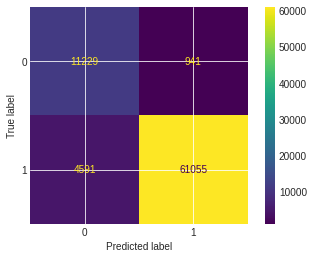
\includegraphics[scale=0.55]{figures/LinearSVC_confusion_matrix.png}
    \caption{Confusion Matrix for the Final SVM model}
    \label{fig:confusion_mat}
\end{figure}

We provide an example of a LIME text explainer for a false negative sample in figures [\ref{fig:fn1}] and a false positive sample in figure [\ref{fig:fp4}], where one can observe the prediction probabilities for each class. Furthermore, the vertical graph presents the contribution of the top ten words regarding class probabilities; these words are also highlighted in the adjacent review text. The blue highlighted words correspond to the probabilities of a negative sentiment of the review, while the words in orange represent probabilities corresponding to the positive sentiment predictions.

\begin{figure*}.
    \centering
    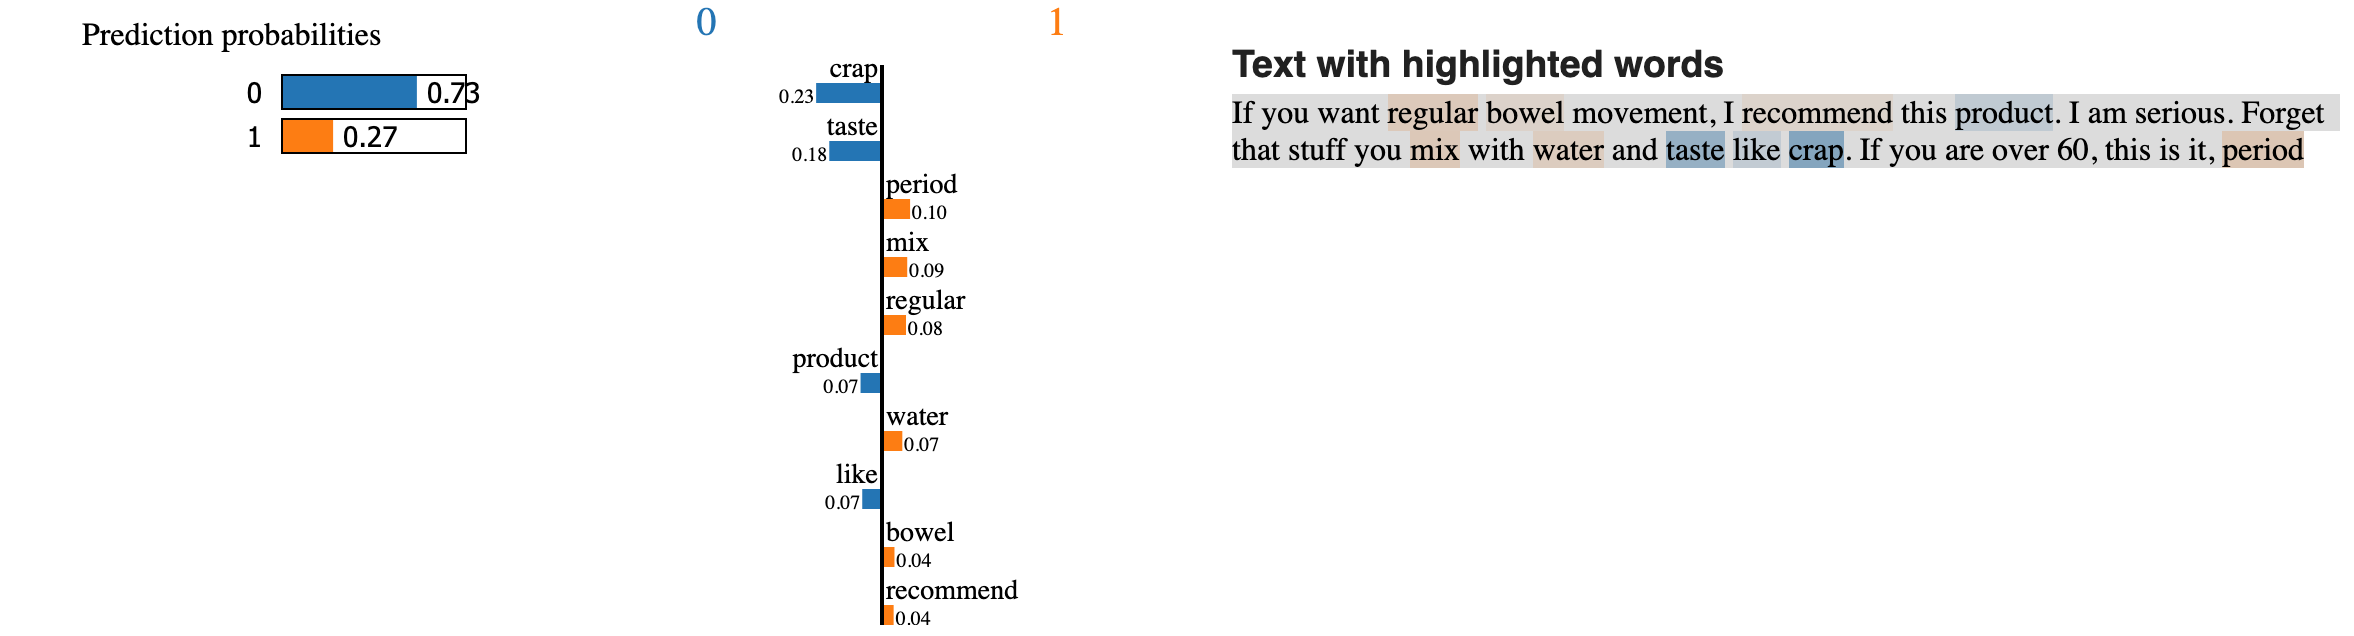
\includegraphics[scale=0.4]{figures/fn1.png}
    \caption{False Negative example, LIME Text Explainer Visualization}
    \label{fig:fn1}
\end{figure*}
\begin{figure*}.
    \centering
    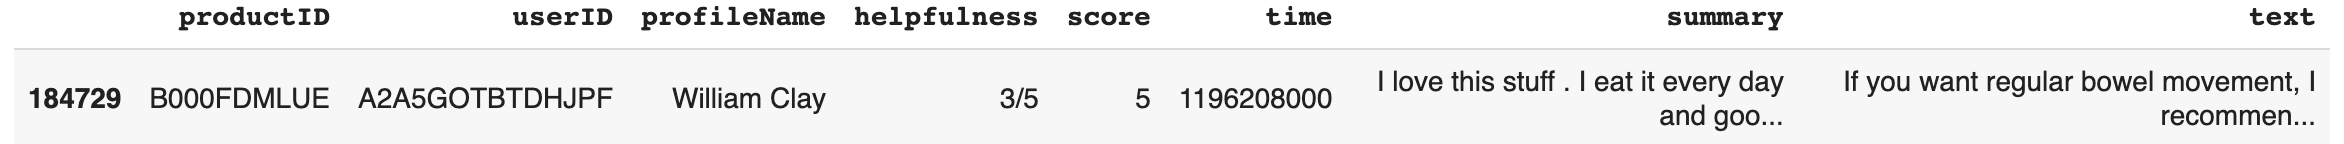
\includegraphics[scale=0.4]{figures/fn1_row.png}
    \caption{False Negative Example, Row Entry from the Test Set}
    \label{fig:fn1_row}
\end{figure*}

\begin{figure*}
    \centering
    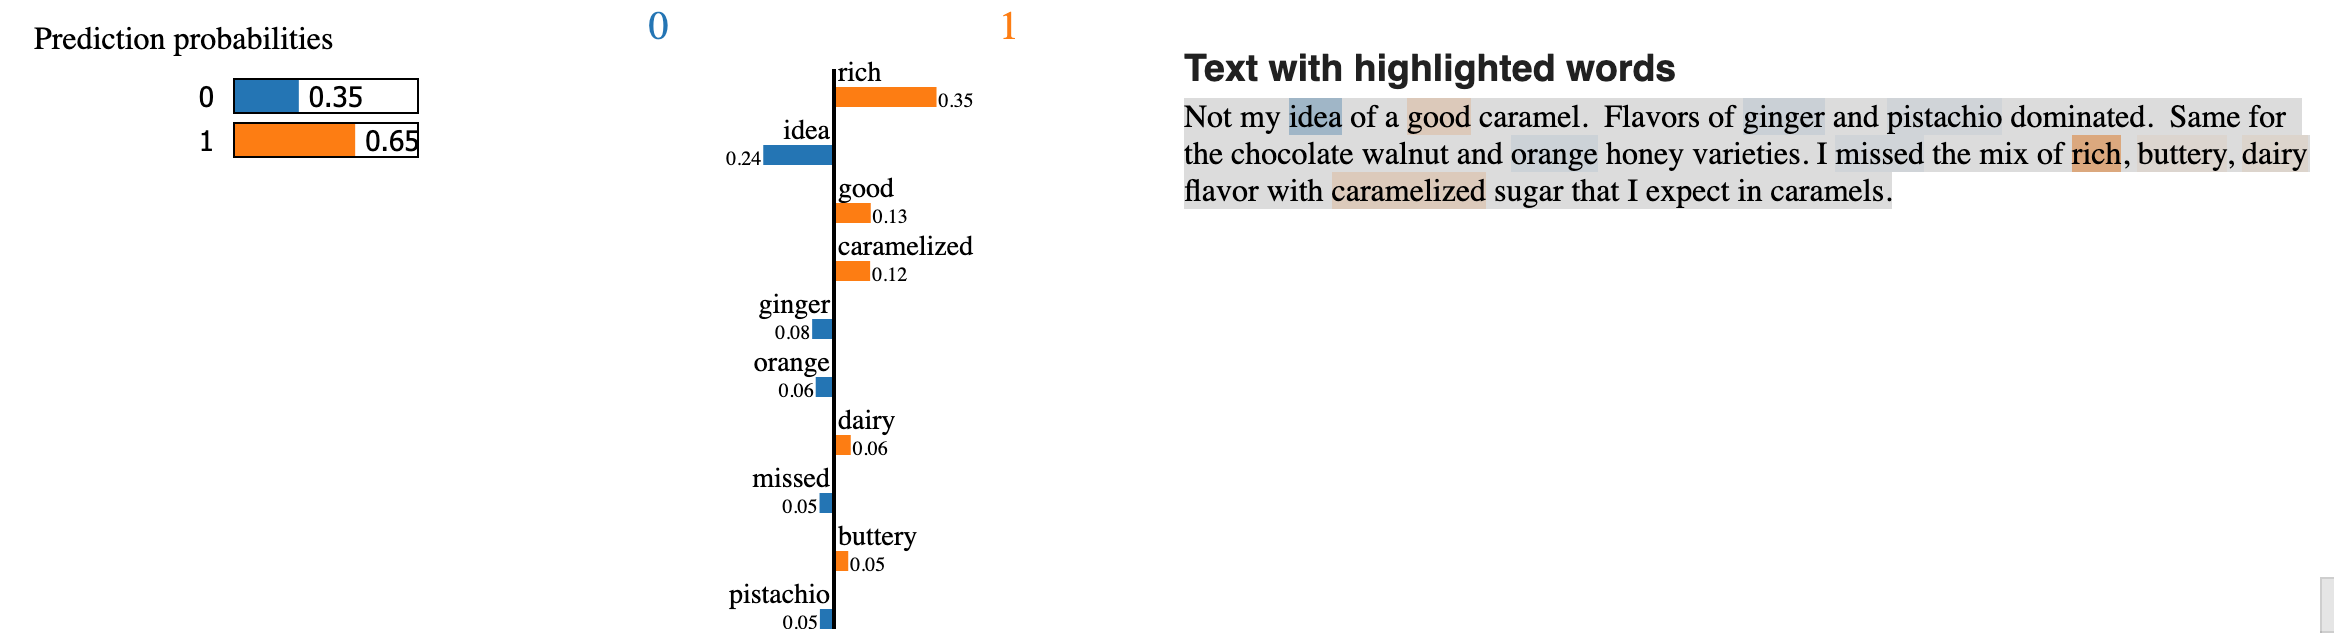
\includegraphics[scale=0.4]{figures/fp4.png}
    \caption{False Positive Example, LIME Text Explainer Visualization}
    \label{fig:fp4}
\end{figure*}
\begin{figure*}
    \centering
    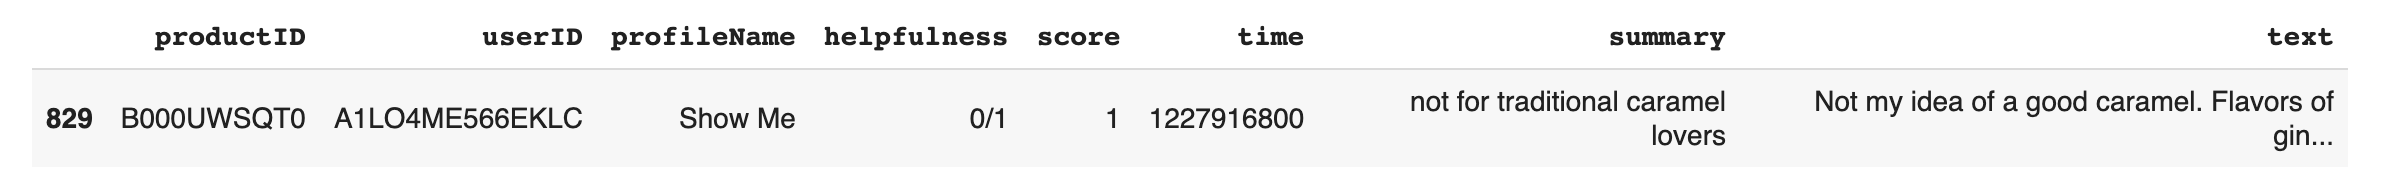
\includegraphics[scale=0.4]{figures/fp4_row.png}
    \caption{False Positive Example, Row Entry from the Test Set}
    \label{fig:fp4_row}
\end{figure*}
 \section{Discussion}

In the first part of the project, we experimented with different classifiers with pipelines created with Count Vectorizer and TfidfVectorizer. These vectorizers are based on the \textit{bag-of-word} idea for the corpus, where the context in the sentence is not considered. However, one can improve the understanding of context by incorporating the \textbf{n-gram} mechanism. In our experiments, with both the vectorizers, using a combination of unigram, bigram (and trigram) instead of just the unigram has improved the model's performance, which can be observed in tables  [\ref{tab:cvec_class_report}] and  [\ref{tab:tfidf_class_report}].

According to Jurafsky and Martin (p.86, 2023), the Logistic Regression model performs better than the Multinomial NB model in larger datasets. The results in the table [\ref{tab:cvec_class_report}] and [\ref{tab:tfidf_class_report}] demonstrate it to be valid to a certain extent. Although the overall accuracy for Multinomial NB and Logistic Regression is almost similar, it is evident that the Precision (and F1-score) for the \textit{negative class} is 2\% to 3\% higher for the Logistic Regression model. As the Precision for the negative class is a ratio of True Negative to the sum of True Negative and False Negative, it can be inferred that the Logistic Regression model is better at minimizing false negatives. The linear SVM model performs slightly better when comparing it with Logistic Regression for both pipelines; it can be observed that Precision for the negative class for linear SVM is 1\% higher than Logistic Regression for both cases. One major limitation of the prediction was relatively poor Precision for the negative reviews across all the experiments caused by higher false negatives. It is important to note that the test set has a class imbalance, with a \textit{positive-to-negative ratio} of approximately \textbf{$5:1$}.

In the next part of the project, we trained the DistilBERT model on the subset of the original training set (20\%) for ten epochs. As per the evaluation metrics in tables [\ref{tab:bert_eval}] and [\ref{tab:bert_distil_class_report}], training and validation accuracies were 0.84 and 0.85 respectively, while the test accuracy was 0.85. However, the F1-score for the negative class was poor (around 0.64), caused by 0.51 precision. The relatively poor evaluation results revealed that the pre-trained DistilBERT model, without the parameter tuning, might not be an ideal choice for sentiment classification. Furthermore, we did not utilize the entire training set for the downstream task, another limitation of this study.

In the third part of the project, we performed LIME analysis for the False Negatives and False Positive samples identified using the tuned Linear SVM model at the end of section [\ref{met:halving_grid}]. Firstly in the figures [\ref{fig:fn1}] and [\ref{fig:fn1_row}], an example of a false negative sample is demonstrated; it can be observed that the words such as \textit{crap} and \textit{taste} overpowers the positive sentiment in the text, resulting in the misclassification. This particular review has a positive summary, and out of five users, three found this helpful, leading us to believe that \textit{summary} of the review could be valuable in  the disambiguation of the edge cases. Next, the figures [\ref{fig:fp4}] and [\ref{fig:fp4_row}]) demonstrate the first False Positive sample, where the model was unable to interpret \textit{Not my idea of a good caramel} as a sentence with negative sentiment, and assigned higher probabilities to words \textit{good}, \textit{rich}, and \textit{caramelized} which classified to be a positive review.

 
 \section{Conclusion}
In this project, we performed a Binary Sentiment Analysis for the Amazon Fine Food Review dataset. In the first part of the project, we experimented with different vectorization techniques and machine-learning classifiers to find a model that delivered the highest performance based on the model evaluation metrics. We used the Halving Grid Search technique with five-fold cross-validation to find the optimum parameters in relatively less time. We observed the Linear SVM model with the TF-IDF vectorization model yielded 93\% accuracy. However, the significant limitation of this method was the lower Precision (0.71) for the negative class (higher false negatives). 

Next, we experimented with DistilBERT for the sentiment classification task and achieved 85\% accuracy. However, the major limitation of this work was the lack of fine-tuning for the DistilBERT model; due to this reason, the Precision for the negative class is relatively poor (0.51). In similar work, the BERT model achieved an accuracy of 79\%. However, it was a five-class classification problem \cite{BERT-finefood}. In future works, we propose to include optimizer scheduling using the 
\texttt{AdamW} \cite{adamw} technique, which could efficiently slow down the learning processing for the initial epochs, leveraging the pre-trained model's knowledge\footnote{\url{https://www.tensorflow.org/text/tutorials/classify_text_with_bert}}. 

Lastly, based on the final Linear SVM model, we performed the LIME technique on the six samples from the test set identified from the misclassified predictions. Several words incorrectly predicted the sentiment of the review \textit{text}, so we propose to use the review \textit{summary} as \textit{prior} class probabilities using the Multinomial NB classifier. Additionally, the review's \textit{helpfulness} could be incorporated as utilized in the works of \cite{helpfulness}. However, we need to conduct more work to evaluate the effectiveness of these changes.



\bibliography{custom}
\bibliographystyle{acl_natbib}

\appendix

\end{document}
